\documentclass{article}

\usepackage{graphicx}
\usepackage{multicol}
\usepackage[margin=0.5in]{geometry}
\usepackage{ragged2e}
\usepackage{boondox-cal}
\renewcommand{\vec}[1]{\mathbf{#1}}

\begin{document}


\title{Calculation of Celestial Bodies using the Fourth Order Runge-Kutta}
\author{Joseph Spear}

\maketitle


\begin{abstract}
\justify
The calculation of the attraction between various bodies is relatively straightforward given only a few bodies. Realistically, there are numerous objects floating around our Solar System, all of which are attracting each other simultaneously through gravitational forces. Every body added increases the number of calculations drastically, and can cause significant likelihood of a human error. Therefore, computational methods are used to calculate the states of the bodies at different times using the Fourth Order Runge-Kutta Approximation technique.
\end{abstract}

\begin{multicols}{2}
\section{Introduction}
Sir Issac Newton famously discovered the phenomenon known as gravity in the late 17th century, discussing the relationship gravity had with the separation between objects in his work known as \textit{Mathematical Principles of Natural Philosophy}. While Newton admitted that his description of gravity was not satisfactory (later expanded upon by Albert Einstein in his work on General Relativity (Schutz)), the simplistic relationship between the force of gravity and the separation would serve an accurate model for many decades. Newton formulated the equation (Halliday, Resnick, 335):

\begin{equation}
    \label{equation1}
    F_g = -G\frac{m_1 \cdot m_2}{\vec{r}^2}
\end{equation}

\vspace{0.1in}

where $F_g$ is the force due to gravity, $G$ is the Gravitational constant, equaling $6.674 \times 10^{-11} \frac{m^3}{kg \cdot s^2}$, $m_1$ and $m_2$ are the masses of the two objects in question, $\vec{r}$ is a vector quantity representing the total separation and direction of the separation between the two objects. Using the principle of superpostion, the forces between multiple bodies can be calculated one at a time, and added together as vector components to find a net force acting on each body.

\section{Fourth Order Runge-Kutta}
The Fourth Order Runge-Kutta Approximation (RK4) method is derived from the simpler but less accurate Euler's method. The approximation method uses four different slope approximations to approximate the next point. By doing this, the run-time of any program using RK4 will be significantly longer, as there are four times more calculations necessary for one step. The standard notation for the RK4 method is as follows:

\begin{equation}
    \label{equation2}
    y_{i+1} = y_i+\frac{\tau}{6}\left(k_1+2k_2+2k_3+k_4\right)
\end{equation}

\vspace{0.1in}

where $k_1$ is an approximation of the slope at the beginning of the step, $k_2$ and $k_3$ are approximations of the slope at the midpoint of the step, and $k_4$ is an approximation of the slope at the end of the step. $\tau$ represents the step, $y_i$ and $y_{i+1}$ represent the position at the original step and the position at the next step respectively. $k_1$ is the initial approximation, and $k_2$, $k_3$, and $k_4$ are terms based on the previous slope approximation.

\section{Implementation}
To calculate the location of various celestial bodies at various points, it is necessary to calculate the acceleration of each body due to every other body. This acceleration will allow us to calculate the next position of the body using either the Verlet Method or the RK4 method. This is done inside a loop with a subroutine as follows:

\begin{verbatim}
do i = 0, numbodies-1
     do j = 0, i - 1
        dx = x(j) - x(i)
        dy = y(j) - y(i)
        dz = z(j) - z(i)

        rmag = sqrt((dx**2) + (dy**2) + (dz**2))
        ax(j) = (-G * m(i) * dx / (rmag**3)) + ax(j) 
        ay(j) = (-G * m(i) * dy / (rmag**3)) + ay(j)
        az(j) = (-G * m(i) * dz / (rmag**3)) + az(j)

        ax(i) = (G * m(j) * dx / (rmag**3)) + ax(i)
        ay(i) = (G * m(j) * dy / (rmag**3)) + ay(i)
        az(i) = (G * m(j) * dz / (rmag**3)) + az(i)
    end do
end do
\end{verbatim}

These calculations allow us to use the approximation methods.

In order to test the power of the approximation methods, the positions, energies, and angular momentum of 249 large celestial bodies are calculated over time. Various different number of steps and changes in time are tested using both the Verlet and RK4 methods.

\section{Results}
To graph the information of the planetary positions, energies, and angular momenta, MATLAB and Gnuplot are used. The following plots are different depictions of the orbits of the planets, sun, and moon in the solar system. The major differences between calculations is the number of steps used to preform the calculation, and the number of days that is being represented.


\begin{center}
\includegraphics[width=3.58in]{SolarSystemFull.eps}
\scriptsize{
Figure 1: Solar System using RK4 Method and 100000 steps
}
\end{center}

Using the RK4 method and plotting every 10 points generated, the shape of the solar system becomes very evident. In this figure, only the sun, 8 planets, Earth's moon, and Ganymede (Jupiter's Moon) are plotted. Even though only 11 bodies are plotted, all 249 bodies have been used to calculate the position, velocity, and acceleration of these bodies over time.

\begin{center}
\includegraphics[width=3.58in]{EarthSunMoon.eps}
\scriptsize{
Figure 2: The Earth, Sun, and Moon over 1 Earth year with 20000 steps
}
\end{center}

In figure 2, the Sun, Earth, and Moon are all plotted over 1 earth year. The Moon is visibly oscillating around the earth over the course of the year as we can observe in reality.

\begin{center}
\includegraphics[width=3.58in]{InnerPlanets_Verlet_20000_5yrs.eps}
\scriptsize{
Figure 3: The Inner Planets using Verlet, 20000 steps, over 5 years
}
\end{center}

\begin{center}
\includegraphics[width=3.58in]{InnerPlanets_RK4_20000_5yrs.eps}
\scriptsize{
Figure 4: The Inner Planets using RK4, 20000 steps, over 5 years
}
\end{center}

Figure 3 and 4 show the Calculated positions of the Inner Planets, Sun, and Earth's moon over the course of 5 years. Figure 3 is using the Verlet Method, and Figure 4 is using the RK4 method with 20,000 steps. While both of the methods are using 20,000 steps, the Verlet method shows a visible error propagation as the orbits of the planets shift with each revolution. The RK4 method proves to much more stable with the same number of steps, as the orbits remain fairly constant.

Other interesting quantities include the Total, Kinetic, and Potential Energies of the system and the Total Angular Momenta. When plotted together the energies show that the addition of the Potential and Kinetic creates the Total Energy which is a constant, with the exception of relatively small calculation errors. This is in line with the Law of Conservation of Energy, as the Total Energy remains relatively constant.

\begin{center}
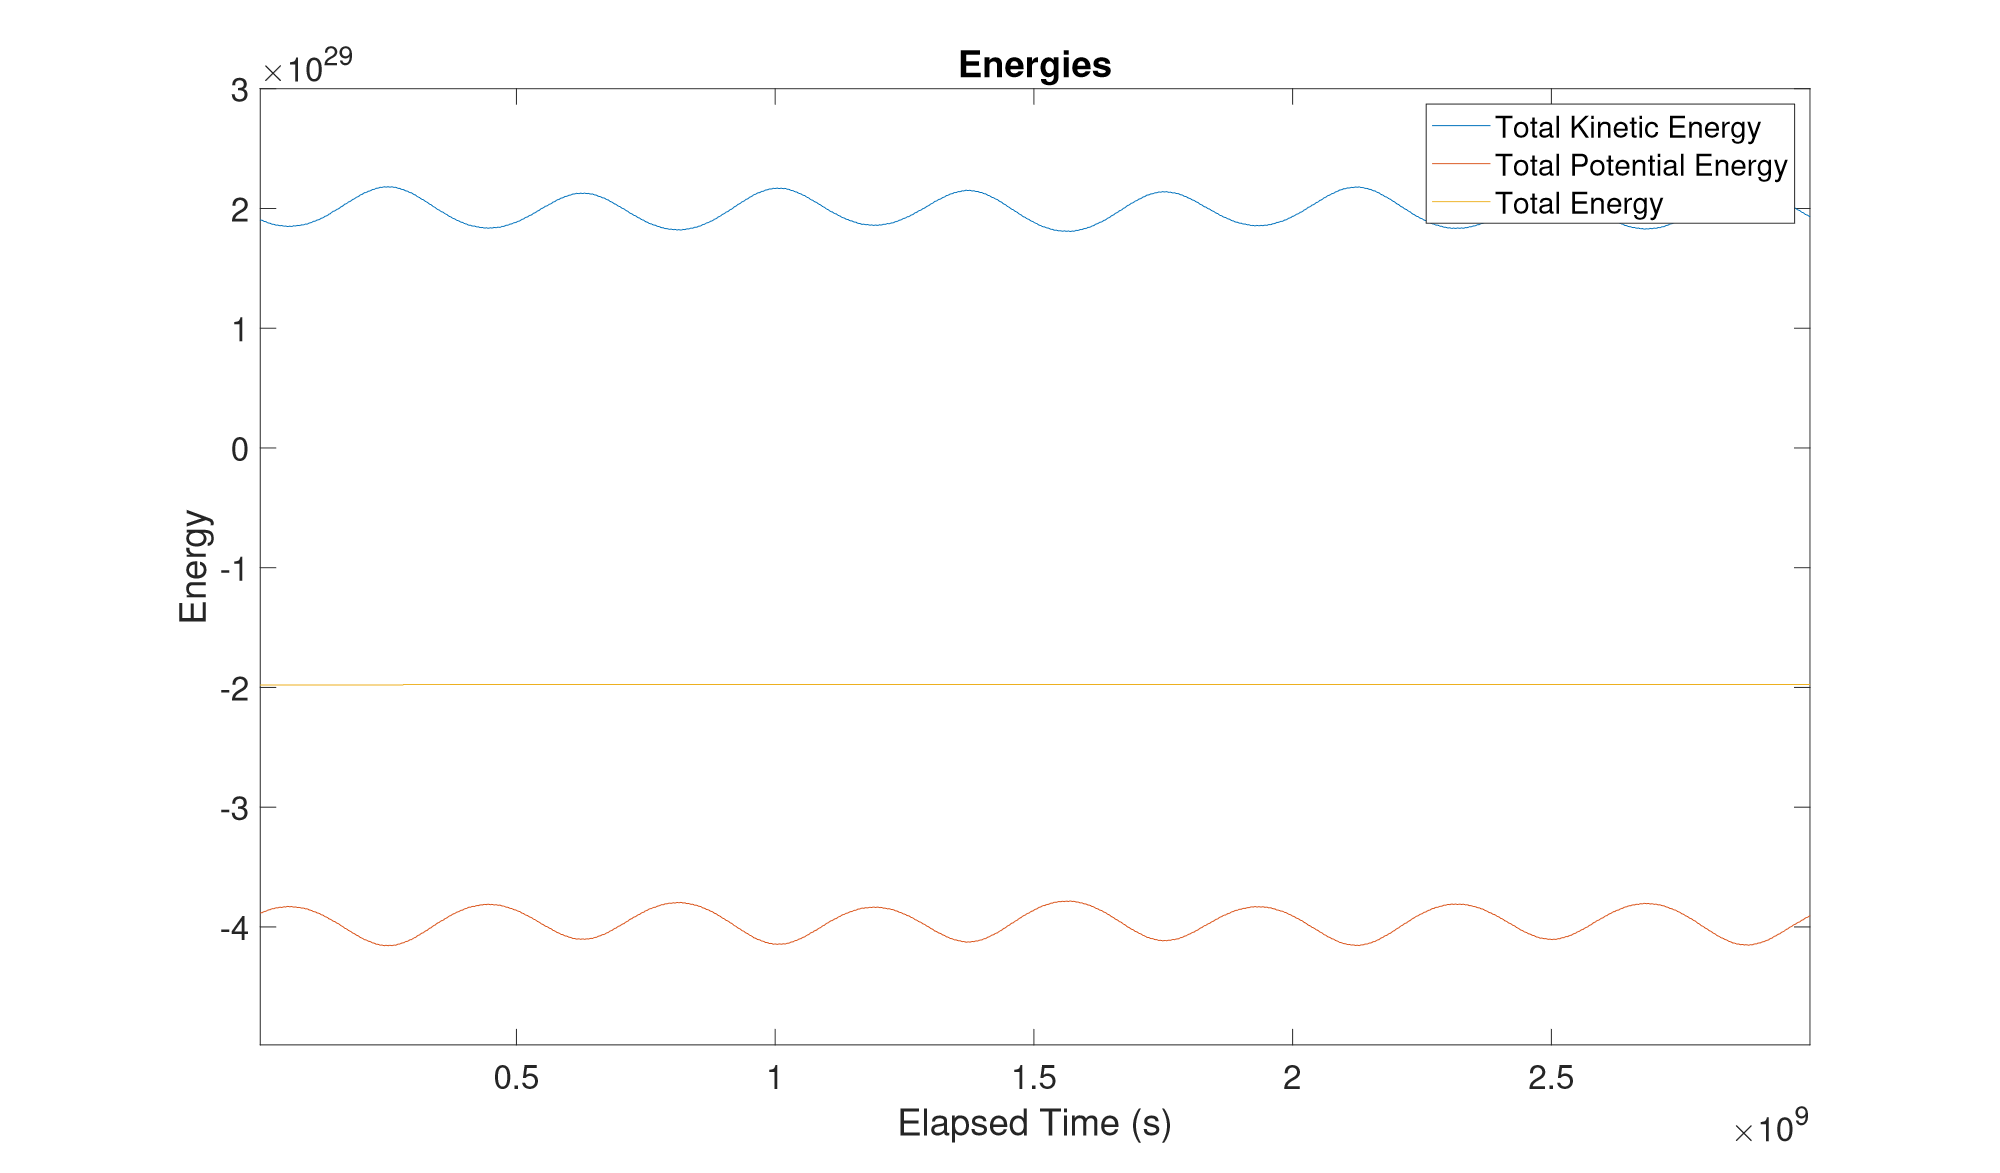
\includegraphics[width=3.58in]{Energies.eps}
\scriptsize{
Figure 5: Total Energies over 100 years with 40000 steps
}
\end{center}

Much like the Conservation of Energy, the Conservation of Angular Momentum states that the Angular Momenta in each direction must also remain constant. This is shown in figure 6 where the Angular Momentum appears constant.

\begin{center}
\includegraphics[width=3.58in]{Momenta.eps}
\scriptsize{
Figure 6: Total Angular Momenta over 100 years with 40000 steps
}
\end{center}


\section{Validation and Verification of the Methods}
One of the challenges with Numerical Methods like Verlet and RK4 is the fact that they become more inaccurate with every step taken. This means that in order to have decent accuracy after many steps, a very small step size must be used. By reducing the step size and increasing the number of steps, the accuracy of the method will improve, however, this takes more computations to successfully perform. Adding computation also adds time, and even with a lot of processing power, large quantities of calculations can increase the run-time of the machine. This creates a trade-off in accuracy versus efficiency and it can determine the numerical method one would use for their analysis.

\begin{center}
\includegraphics[width=3.58in]{ErrorVsRun_11713.eps}
\scriptsize{
Figure 7: Average Error and Run Time for 11,713 days
}
\end{center}

\begin{center}
\includegraphics[width=3.58in]{ErrorVsRun_6752.eps}
\scriptsize{
Figure 8: Average Error and Run Time for 6,752 days
}
\end{center}

\begin{center}
\includegraphics[width=3.58in]{ErrorVsRun_4235.eps}
\scriptsize{
Figure 9: Average Error and Run Time for 4,235 days
}
\end{center}

Figures 7, 8, and 9 display the error versus the time it takes to run the numerical method. To calculate the error, the actual data of the planets after the indicated days are taken from the JPL Horizons program (https://ssd.jpl.nasa.gov/horizons.cgi) and contrasted with the data produced from the numerical method. For each run, the average error is calculated for every planet and summed up to produce the final error estimate. The runtime for the numerical approximation is the difference between the system time before the calculation and the system time after the calculation finishes using the built in FORTRAN function cpu\_time.

One possibility to improve the run time is by using multiple threads. By doing this, the runtime may be use significantly reduced as the computer is multi-tasking with the work that it is being asked to do. Multi-threading is not implemented in 

\section{Conclusion}
When deciding which Numerical Method to use, it is important to take into consideration the error that will be produced and the runtime that will be needed. More accurate methods lead to quicker solutions implementation-wise, but will take longer to run, while a less accurate method may be used (and will be needed) for many more steps with less time per step to approximate the same model. This computational experiment proves that the RK4 method is much more accurate over long periods of time, while the Verlet method is faster. In all cases, the RK4 method took more time than the Verlet method.
\section{References}

\begin{enumerate}

\item Park, Ryan S. NASA's Jet Propulsion Laboratory, 2019, https://ssd.jpl.nasa.gov/horizons.cgi. Accessed 7 Oct. 2019.

\item Schutz, Bernard \textit{A First Course in General Relativity} Cambridge, UK, Cambridge University Press, 2009.

\item Halliday, Resnick \textit{Fundamentals of Physics} Danvers, MA, John Wiley, 2014.

\end{enumerate}

\end {multicols}
\end{document}